\documentclass[tikz,border=8pt]{standalone}
% Shared look for every TikZ diagram. Load with \input{../../tools/tikz-style.tex}
\usepackage[T1]{fontenc}
\usepackage{lmodern}
\renewcommand{\sfdefault}{lmr}  % diagrams use the same serif as the text
\usetikzlibrary{arrows.meta, positioning, shapes.geometric, calc, fit, backgrounds}
\definecolor{cblue}{HTML}{4C78A8}
\definecolor{corange}{HTML}{F58518}
\definecolor{cgreen}{HTML}{54A24B}
\definecolor{cred}{HTML}{E45756}
\definecolor{cpurple}{HTML}{B279A2}
\definecolor{cgrey}{HTML}{6B6B6B}
\tikzset{
  every picture/.style={font=\sffamily, line width=1.2pt},
  box/.style={draw=#1, fill=#1!12, rounded corners=4pt, align=center, inner sep=7pt, minimum height=1.1cm},
  box/.default=cgrey,
  arrow/.style={-{Stealth[length=3mm]}, draw=cgrey, line width=1.4pt},
  title/.style={font=\sffamily\bfseries\Large},
  note/.style={font=\sffamily\small, text=cgrey, align=center},
}
\AtBeginDocument{\hyphenpenalty=10000 \exhyphenpenalty=10000}

\begin{document}
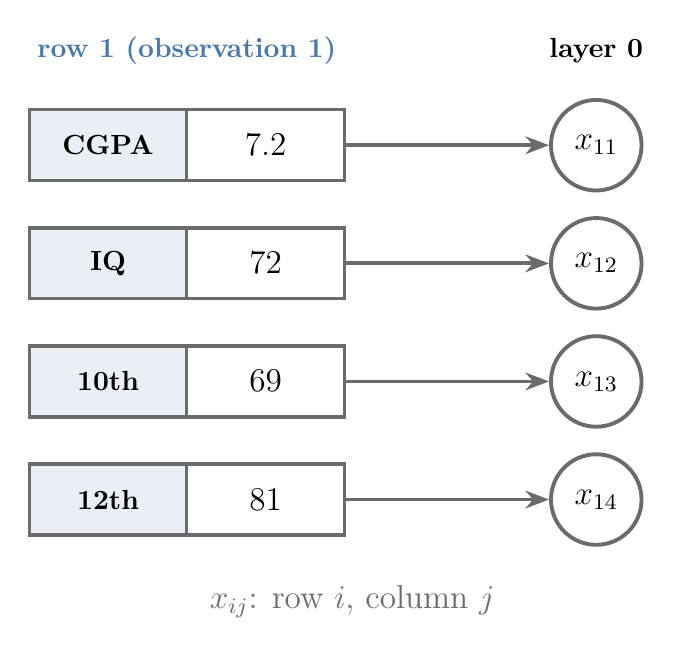
\begin{tikzpicture}[every node/.append style={font=\sffamily\large},
  cell/.style={draw=cgrey, minimum width=2.0cm, minimum height=0.9cm},
  inp/.style={circle, draw=cgrey, fill=white, minimum size=1.15cm, line width=1.4pt}]
  \foreach \j/\h/\v in {1/CGPA/7.2, 2/IQ/72, 3/10th/69, 4/12th/81} {
    \node[cell, fill=cblue!12, font=\sffamily\bfseries] (h\j) at (0, 3.6-1.5*\j+0.9) {\h};
  }
  \foreach \j/\h/\v in {1/CGPA/7.2, 2/IQ/72, 3/10th/69, 4/12th/81} {
    \node[cell] (v\j) at (2.0, 3.6-1.5*\j+0.9) {\v};
    \node[inp] (x\j) at (6.2, 3.6-1.5*\j+0.9) {$x_{1\j}$};
    \draw[arrow] (v\j) -- (x\j);
  }
  \node[font=\sffamily\bfseries, text=cblue] at (1.0, 4.2) {row 1 (observation 1)};
  \node[font=\sffamily\bfseries] at (6.2, 4.2) {layer 0};
  \node[note, font=\sffamily\large] at (3.1, -2.8) {$x_{ij}$: row $i$, column $j$};
\end{tikzpicture}
\end{document}
